\documentclass{standalone}

\usepackage{pgfplots}

\begin{document}
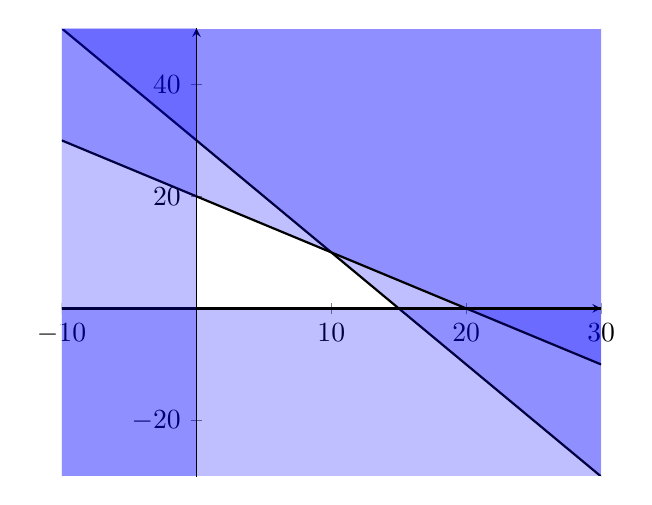
\begin{tikzpicture} 

    \begin{axis}[enlargelimits=0.1, axis lines=middle]
    % First one
    \addplot [color=white,fill=blue, 
              fill opacity=0.25]coordinates {
              (-10,50)
              (30,50)
              (30,-30)};
    \addplot[domain=-10:30,fill=gray!50, thick] {30 - (2*x)};
    % Second one
    \addplot [color=white,fill=blue, 
              fill opacity=0.25]coordinates {
              (-10,30)
              (-10,50)
              (30,50)
              (30,-10)};
    \addplot[domain=-10:30,fill=gray!50, thick] {20 - x};
    % Third one
    \addplot [color=white,fill=blue,
              fill opacity=0.25]coordinates {
              (30,-30)
              (-10,-30)
              (-10,0)
              (30,0)};
    \addplot[domain=-10:30,fill=gray!50, thick] {0};
    \addplot [color=white,fill=blue,
              fill opacity=0.25]coordinates {
              (-10,50)
              (-10,-30)
              (0,-30)
              (0,50)};
    \addplot[fill=gray!50, thin] coordinates {
              (0,-30)
              (0,50)};
    \end{axis}
\end{tikzpicture}  
\end{document}